\chapter{Implementation}

\section{Introduction}
% Purpose: Briefly state the chapter's purpose (detailing the implementation of Parallax), reiterate the core goal (automatic parallelism via INs), and outline the chapter's structure (compiler pipeline, runtime, tooling).
% Questions:
% - What is the main achievement described in this chapter? (e.g., "This chapter details the implementation of the Parallax compiler and parallel runtime...")
% A: Infer from introduction
% - What is the core technical approach? (...which enables automatic parallelism by compiling a functional language to interaction nets.")
% A: Infer from introduction
% - What are the major components covered? (e.g., "We will cover the compiler pipeline stages, the parallel runtime architecture based on partition ownership, GC integration, and supporting tooling.")
% A: Infer from crates/README.md
This chapter details the concrete implementation of the Parallax compiler and parallel runtime, built to achieve the central goal of automatic, efficient parallelism by compiling a high-level functional language to interaction nets. We will describe the journey from source code to execution, covering every stage of the compiler pipeline.

\section{Repository Overview}
% Purpose: Describe the high-level structure of the source code repository, identify key crates and external dependencies, and explain the rationale for using specific tools/libraries. Acknowledge that the project was built from scratch. Fulfills a specific mark scheme requirement.
% Questions:
% - Was the code written from scratch?
% A: Yes
% - How is the codebase organized? (Multi-crate Cargo workspace?)
% A: Infer from crates/README.md, but yep exactly
% - What are the main crates and their roles? (List `parallax-source`, `syntax`, `resolve`, `types`, `hir`, `mir`, `native`, `codegen`, `net`, `rt`, `db`, `cli`, `tree-sitter-parallax`. Briefly describe each's function in the pipeline/system. Maybe use a table?)
% A: Infer from crates/README.md. If possible to a full diagram, that'd be great
% - What are the most important external libraries/tools used? (Tree-sitter, Salsa, Cranelift, Crossbeam, rsgc, repc, clap, miette, parking_lot, slab, etc.)
% A: All of those. If I remember more I can add them in later.
% - Why were these specific external tools/libraries chosen? (Justify based on capabilities, e.g., Salsa for incrementality, Cranelift for JIT/Rust integration, Crossbeam for concurrency primitives.)
% A: Maybe we get to that in later chapters? There are a lot of dependencies so maybe listing things outside of salsa, miette, clap and thiserror might be a bit much.
The entire Parallax codebase was developed from scratch for this project.

\begin{figure}[h!]
    \centering
\begin{verbatim}
parallax/
├── Cargo.toml            # Workspace definition
├── README.md             # Top-level project description
├── crates/               # Directory containing core implementation crates
│   ├── ...
│   ├── parallax-cli/     # Command-line interface
│   |   ├── src/          # Source code
│   |   ├── tests/        # Tests
│   |   ├── Cargo.toml    # Cargo configuration
│   └── ...               # Other crates (MIR, Backends, Runtime)
├── ...                    # Other files (tests, docs, etc.)
\end{verbatim}
    \caption{Parallax Project Directory Structure}
    \label{fig:impl_dir_structure}
\end{figure}

This structure promotes modularity and separates the distinct phases of the compiler and runtime system.

\subsection{The CLI: \texttt{parallax-cli}}
% Purpose: Describe the user-facing CLI, its commands, argument parsing (clap), and error reporting (miette).
% Questions:
% - What is the overall goal of the CLI's design? (UX, familiarity)
% - How are commands defined and parsed? (clap Subcommands, Parser derive)
% - What are the key commands? (`new`, `build`, `run`, `check`, etc.)
% - How are errors reported to the user? (miette Diagnostic derive, CliError enum)
% - How does it interact with the core compiler? (Calls into parallax-db)

The user's primary interaction with Parallax is via the command-line interface (CLI) in the \texttt{parallax-cli} crate. It's designed for a familiar user experience for those who have used Cargo, offering intuitive commands and clear diagnostics.

\subsubsection{Command Structure and Parsing}

The CLI uses the \textbf{\texttt{clap}} library \cite{Clap} for command structure and argument parsing. The main \texttt{plx} command and its subcommands are defined using \texttt{clap::Parser} derive macros. This automatically generates help output below.

\begin{figure}[h!]
    \centering
    \begin{verbatim}
Parallax Compiler

Usage: plx [OPTIONS] <COMMAND>

Commands:
  new     Create a new Parallax frame (project)
  init    Initialize a Parallax frame in an existing directory
  build   Compile the current frame
  run     Compile and run the current frame
  check   Analyze the current frame and report errors, without building
  help    Print this message or the help of the given subcommand(s)

Options:
  -v, --verbose...  Increase logging verbosity
  -q, --quiet...    Decrease logging verbosity
  -h, --help        Print help
  -V, --version     Print version
    \end{verbatim}
    \caption{Output of $\texttt{-{}-help}$}
    \label{fig:impl_cli_help}
\end{figure}

\subsubsection{Error Reporting}

To provide high-quality diagnostics, the entire pipeline leverages the \textbf{\texttt{miette}} library \cite{Miette}.


\begin{figure}[h!]
    \centering
    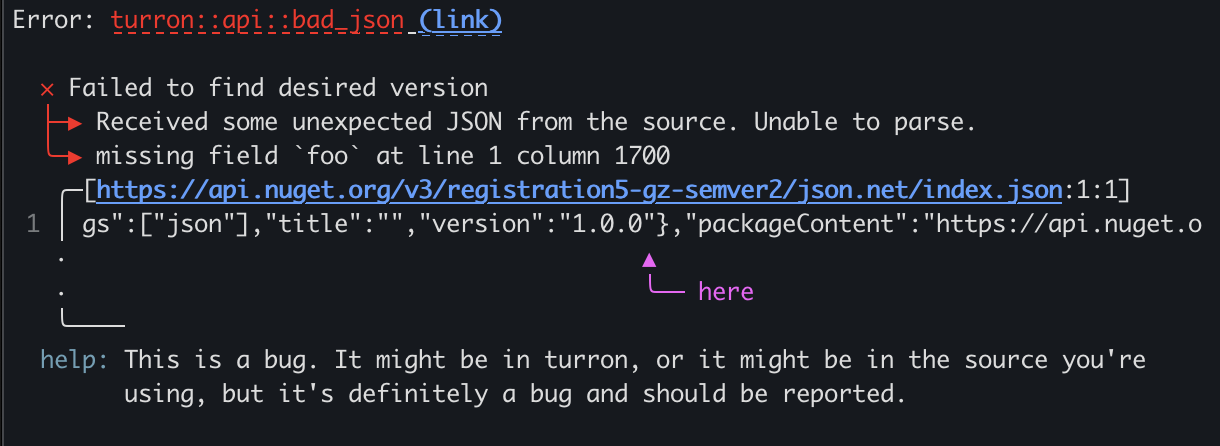
\includegraphics[width=0.8\textwidth]{images/miette-example.png}
    \caption{Example of a Miette diagnostic report showing source context.}
    \label{fig:impl_miette_example}
\end{figure}

All error types derive \texttt{miette::Diagnostic}, allowing errors to be richly annotated with error codes, severity levels, contextual help messages and even source code snippets with labelled spans indicating the part of the source code that fails to compile.

\subsection{Incremental Compilation: \texttt{parallax-db}}

While the CLI provides the user interface, the compilation is orchestrated by \texttt{parallax-db}. This crate establishes the foundation for incremental compilation using the \texttt{Salsa} library \cite{Salsa}, crucial for a responsive developer experience by avoiding full recompilations for minor changes.

\subsubsection{Salsa Framework Overview}

Salsa \cite{Salsa} achieves incrementality through a query-based system centered around a database. Compiler passes are modelled as tracked queries (functions) that operate on this database. Base data, such as the content of source files, are treated as inputs. 

When a tracked query executes, Salsa performs dependency tracking, recording which inputs or other tracked queries it accessed. The result of the query is then cached. When an input changes (e.g., a file is edited), Salsa marks it and any dependent query results as potentially stale through a process called invalidation. 

The next time a query marked as potentially stale is needed, Salsa first checks if its direct dependencies actually produced a different output compared to the last run. If the dependencies' outputs are identical despite the underlying input change, the cached result is still valid and returned without re-executing the query. Otherwise, the query re-executes. This demand-driven, memoized approach ensures only the necessary parts of the compilation pipeline run after a change.

\section{Parsing, Name Resolution, and Type Checking}
% Figure for Frontend Pipeline
\begin{figure}[h!]
    \centering
    \begin{tikzpicture}[node distance=0.5cm and 1.5cm, auto, >=Latex, % Adjusted node distance
        stage/.style={rectangle, draw, text centered, rounded corners, minimum height=3em, text width=10em, align=center}, % Increased min height
        arrow/.style={->, thick}]
    
        % Top row nodes
        \node (source) [stage] {Source Files \\ (.plx, frame.toml)};
        \node (frame) [stage, right=of source] {Concrete \\ Syntax Tree (CST)};
        \node (ast) [stage, right=of frame] {Abstract \\ Syntax Tree (AST)};
    
        % Bottom row nodes
        \node (resolved_ast) [stage, below=of ast] {Resolved AST};
        \node (typed_ast) [stage, left=of resolved_ast] {Typed AST};
        \node (hir) [stage, left=of typed_ast] {HIR};
    
        % Arrows
        \draw [arrow] (source.east) -- (frame.west);
        \draw [arrow] (frame.east) -- (ast.west);
        \draw [arrow] (ast.south) -- (resolved_ast.north);
        \draw [arrow] (resolved_ast.west) -- (typed_ast.east);
        \draw [arrow] (typed_ast.west) -- (hir.east);
    
    \end{tikzpicture}
    \caption{Parallax Frontend Pipeline Stages}
    \label{fig:impl_pipeline}
\end{figure}

The first phase of the Parallax compiler involves transforming the raw source code files into a structured, resolved, and typed representation suitable for intermediate representation generation.

\subsection{Source Management: (`parallax-source`)}
% Purpose: Describe how source files and project configuration (`frame.toml`) are loaded and managed incrementally using Salsa.

The compilation process begins with the \texttt{parallax-source} crate, responsible for discovering, loading, and managing the source code and configuration of a Parallax project, referred to as a "Frame", using the \texttt{SourceDatabase} trait integrated into the main `Compiler` database. A Frame represents a single compilation unit, conceptually similar to a crate in Rust or a package in other ecosystems.

Each Frame is defined by a configuration file, typically named \texttt{frame.toml}, located at the root of the project directory. This file, parsed using the \texttt{toml} and \texttt{serde} crates, specifies essential metadata such as the package name, version, entry point (usually \texttt{src/main.plx}), and crucially, its dependencies on other Frames (currently supporting local path dependencies). 

The primary entry point for discovering and loading project sources is the \texttt{load\_frame} tracked query. This returns a \texttt{Frame} tracked struct, which encapsulates the frame configuration, the root directory structure, all discovered source files, and the same for all dependency \texttt{Frame}s, providing a complete view of the project's sources for subsequent compiler stages.

\section{Parsing: \texttt{parallax-syntax}}

The compilation process enters the parsing stage with the \texttt{parallax-syntax} crate, which transforms the raw source code text into a structured Abstract Syntax Tree (AST).

\subsection{Language Design and AST Representation}

As established during preparation (Section~\ref{sec:prep_requirements}), the surface syntax of Parallax is heavily inspired by Rust. This choice was made deliberately to leverage Rust's familiarity among systems programmers, its expressive type system features, and its generally well-regarded design principles. The goal was to provide a productive and comfortable environment for developers, reducing the learning curve typically associated with novel parallel programming models.

While the semantics are functional and tailored for interaction net compilation, the syntax aims for clarity and expressiveness. Key features include algebraic data types, pattern matching, generics, and trait-based polymorphism, all presented with Rust-like syntax. The following sample code provides a brief tour of the language's core syntactic elements, illustrating its resemblance to Rust:

\begin{lstlisting}[language=Rust, caption={Parallax Language Syntax Tour}, label={lst:impl_syntax_tour}]
// Variables (immutable by default)
let x = 42;               // Type inferred
let pi: f64 = 3.14;      // Explicit type

// Basic control flow
let status = if connected then "online" else "offline";
let message = get_message();
match message {
    Message::Quit => (),
    Message::Write(s) => println(s),
    Message::Move { x, y } => move_cursor(x, y)
}

// Functions
fn greet() = println("Hello, world!");

// Structs
struct Point { x: f64, pub y: f64 }
impl Point {
    pub fn new(x: f64, y: f64) -> Self = Point { x, y };
    pub fn distance(self, other: Point) -> f64 = { ... };
}

// Enums
enum Option<T> { Some(T), None }


// Explicit Sequencing
log("Start") -> process() -> log("End");

// Generics and Traits
struct Pair<T> { first: T, second: T }
trait Display { fn display(self) -> String; }
fn print<T: Display>(value: T) = println(value.display());
\end{lstlisting}

\subsection{Parsing Implementation}

The technical implementation relies on the \texttt{tree-sitter} parsing library, chosen for its robust error handling and support for incremental parsing. \texttt{parallax-syntax} uses a custom Tree-sitter grammar (in \texttt{tree-sitter-parallax}) to process source file text into an initial Concrete Syntax Tree (CST).

This CST is then traversed to build Parallax's AST. During this conversion, structural checks are performed and errors (from both Tree-sitter and the conversion) are collected. Crucially, AST nodes retain \texttt{miette::SourceSpan} information from the CST, enabling precise diagnostics using the unified \texttt{SyntaxError} type and \texttt{miette} \cite{Miette}.

\subsection{Name Resolution: \texttt{parallax-resolve}}

While the AST represents grammatical structure, the compiler needs semantic understanding. The \texttt{parallax-resolve} crate builds this understanding by resolving names to unique definitions (represented by a \texttt{Symbol}), considering scope and imports. This critical stage bridges the syntactic AST and the type checker, focusing primarily on resolving item signatures and module structure rather than full type checking of expressions.

This resolution process involves multiple coordinated passes over the project structure, orchestrated via the \texttt{ResolveDatabase} trait and \texttt{Salsa} queries for incrementality:

\subsubsection{1. Definition Collection}
An initial inventory pass identifies all definitions (functions, structs, enums, traits, etc.) across the root frame and its dependencies, assigning each a unique \texttt{Symbol}. Basic information (name, parent, visibility, location) is stored in a central \texttt{DefinitionInfo} map. The standard library AST is integrated during this pass.

\subsubsection{2. Scope Building and Import Resolution}
Next, the resolver determines name visibility within each module. It builds a hierarchical \texttt{ModuleScope} for each module, initially containing local definitions. It then processes \texttt{use} declarations, resolving paths relative to the current module and other module scopes. This handles simple paths, aliases, group imports, and globs, adding entries mapping imported names to resolved \texttt{Symbol}s in the relevant scope. If a path remains unresolved, the standard library prelude (\texttt{std::prelude}) is checked as a fallback.

\subsubsection{3. Type Signature Resolution}
Using the definition map and module scopes (including imports and prelude), this pass interprets type annotations in item signatures (e.g., function parameters, return types, struct fields), resolving type names like \texttt{MyStruct} or \texttt{Option<T>} to \texttt{types::ResolvedType} structures.

\subsubsection{4. Expression and Function Body Resolution}
Finally, the resolver traverses function and method bodies. It uses a \texttt{ScopeStack} to track local variables from parameters and \texttt{let} bindings. When resolving names in expressions, it checks the local stack first, then the module scope, then the prelude. This pass handles basic name resolution within expressions, deferring complex type inference and trait solving to \texttt{parallax-types}.

\subsubsection{5. Output}

The final output is the \texttt{\#[salsa::tracked] ResolvedModuleStructure}, containing all definitions with resolved signatures and expression trees, ready for type checking.

\subsection{Standard Library: \texttt{parallax-stdlib}}

Like most languages, Parallax has a standard library (\texttt{std}) providing essential types, traits, and functions. These are defined in the \texttt{parallax-stdlib} crate.

\subsubsection{Implementation and Integration}

The standard library is implemented as standard \texttt{.plx} source files containing familiar definitions (\texttt{Option}, \texttt{Result}, \texttt{Add}, \texttt{println}, etc.). These files are embedded directly into the compiler using Rust's \texttt{include\_str!} macro. A dedicated Salsa query creates a \texttt{Frame} object from these sources, which is then processed like any other dependency during compilation, making its items available seamlessly.

\subsubsection{Contents}

The standard library provides foundational elements like basic data structures (\texttt{Option}, \texttt{Result}), standard traits for operator overloading (\texttt{Add}, \texttt{Sub}, \texttt{PartialOrd}), conversion traits (\texttt{Into}, \texttt{TryInto}), and basic I/O functions (\texttt{println}). It also defines compiler \textbf{intrinsics} for fundamental operations (primitive arithmetic, I/O, panic) whose implementations are provided by later compiler stages.

\subsubsection{Prelude}

For convenience, commonly used items (\texttt{Option}, \texttt{Result}, \texttt{Vec}, \texttt{String}, common traits) are exported via \texttt{std/prelude.plx}. The name resolver automatically checks this prelude scope as a fallback, making these items available without explicit imports.

\section{Type Checking: \texttt{parallax-types}}

With names resolved to symbols and signatures understood, the \texttt{parallax-types} crate performs the crucial task of full semantic validation. It takes the output produced by \texttt{parallax-resolve} and verifies that the code adheres to the language's type system rules, inferring types where necessary and resolving trait implementations.

\subsection{Type Inference and Unification}

To reduce the burden of explicit type annotations, Parallax employs a type inference system based on the principles of the Hindley-Milner (HM) algorithm \cite{Hindley1969}. The core idea of HM is to automatically deduce the most general type for an expression or function without requiring explicit type declarations from the programmer, while still ensuring type safety. Parallax adapts this using a bidirectional approach, combining top-down type checking (when an expected type is known) with bottom-up inference (when it is not).

The central mechanism is \textbf{unification}, managed by the \texttt{InferenceContext}. When the type of an expression is initially unknown (e.g., a variable bound in a \texttt{let} statement like \texttt{let x = ...}), the type checker assigns it a fresh \textbf{inference variable} (represented internally as \texttt{TyKind::Var}), essentially a placeholder for an unknown type.

As the checker traverses expressions, it generates type constraints based on how values are used. For example, if a variable \texttt{x} (assigned inference variable \texttt{t0}) is added to an integer literal (type \texttt{i32}), the checker generates a constraint like \texttt{t0 = i32}. The \texttt{unify} method within the \texttt{InferenceContext} attempts to solve these constraints by finding a consistent \textbf{substitution} (a mapping from inference variable IDs to concrete types or potentially other inference variables). If unification succeeds, the substitution is applied, progressively refining the inferred types of variables. If unification fails (e.g., trying to unify \texttt{i32} and \texttt{bool}), a \texttt{TypeError::TypeMismatch} is reported.

This process allows the compiler to infer types in many common scenarios, such as local variable bindings and function return types, striking a balance between explicit annotation and automatic deduction. While unification resolves constraints for concrete types and inference variables, handling generic definitions requires an additional step.

\subsection{Generic Instantiation}

Generic definitions (like \texttt{fn id<T>(x: T)}) contain type parameters. Before use in a concrete context (like \texttt{id(42)}), the generic type is \textbf{instantiated} by replacing parameters with fresh inference variables (e.g., \texttt{fn(t0) -> t0}). Unification then determines the specific types for that usage (e.g., \texttt{t0} becomes \texttt{i32}).

\subsection{Trait Solving}

Parallax uses rust-style traits for ad-hoc polymorphism. Trait solving resolves trait obligations based on inference and instantiation.

\subsubsection{Trait Bounds}

When a generic function or type definition includes a bound like \texttt{<T: Add>}, the checker must verify this constraint. At call sites or instantiation points, after generic instantiation replaces \texttt{T} with a concrete type or an inference variable, the checker ensures that this resulting type actually provides an implementation for \texttt{Add}. This often involves looking up implementations in the \texttt{TraitRepository} and may trigger further unification if the implementation itself is generic.

\subsubsection{Handling Associated Types}

Traits can define associated types (e.g., \texttt{trait Iterator { type Item; ... }}). When checking an \texttt{impl} block, the compiler ensures that concrete types are provided for all associated types defined by the trait. When using a trait bound (like \texttt{<I: Iterator>}), the compiler can then refer to these associated types (e.g., \texttt{I::Item}) and substitute the concrete type provided by the specific implementation found for \texttt{I} during trait solving.

Overall, trait solving relies heavily on the information gathered during name resolution about defined traits and \texttt{impl} blocks. It frequently interacts with the unification engine, especially when dealing with generic implementations, to find a consistent match between the required trait and the available implementations for a given type.

\subsubsection{Method Dispatch}

Trait solving is also essential for method calls. When a method call occurs (e.g., \texttt{vec.push(1)}), Parallax performs \textbf{static dispatch}. The checker first determines the concrete type of the receiver (the value before the dot, here \texttt{Vec<i32>} after potential inference). It then looks up the method name (\texttt{push}) specifically for that type. The lookup prioritises \textbf{inherent methods} (those defined directly in an \texttt{impl Vec<i32>} block, if applicable) before searching for methods provided by traits implemented for \texttt{Vec<i32>}.

The \texttt{TraitRepository}, populated during the checking of all \texttt{impl Trait for Type} blocks, is the central registry for finding trait method implementations. The checker queries the repository to find the unique, applicable trait implementation (\texttt{impl SomeTrait for Vec<i32>}) that provides the required method (\texttt{push}). Successful resolution links the method call directly to the specific underlying function symbol defined in the inherent or trait \texttt{impl} block at compile time, avoiding the runtime overhead associated with dynamic dispatch mechanisms like vtables.

\subsection{Expression and Definition Checking}

The mechanisms described above -- inference, unification, generic instantiation, and trait solving -- culminate in the comprehensive checking of function bodies and item definitions. The checker recursively traverses the \texttt{ResolvedExpr} trees within function bodies. For each node (binary operation, function call, \texttt{if} expression, \texttt{match} expression, etc.), it applies the relevant typing rules, performs unification to enforce consistency, instantiates generics as needed, resolves trait methods, and generally ensures semantic correctness according to the language rules. For example, it verifies that the condition of an \texttt{if} is boolean, that the operands of \texttt{+} support the \texttt{Add} trait, and that the types of \texttt{match} arms are compatible.

The output of this recursive traversal is a \textbf{\texttt{TypedExpr}} tree, where each node is annotated with its fully inferred or checked type (\texttt{Ty}). Concurrently, the checker verifies the internal consistency of definitions themselves (e.g., ensuring struct fields have valid types, checking trait implementations against trait definitions).

\subsection{Output}

The final result is the \texttt{\#[salsa::tracked] TypedModule} struct, containing fully typed definitions and the resolved \texttt{TraitRepository}. This validated representation serves as input for HIR generation.

\section{High-level IR: \texttt{parallax-hir}}

After the frontend stages validate the program's structure and semantics, producing a fully typed representation (\texttt{TypedModule}), the compiler enters the intermediate representation phase. The first crucial IR is the High-level Intermediate Representation (HIR), generated by the \texttt{parallax-hir} crate. This section details the HIR's design, the process of lowering to it, its advantages, and the optimizations performed at this level.

\subsection{Administrative Normal Form (ANF)}

Parallax's HIR is specifically designed around \textbf{Administrative Normal Form (ANF)} \cite{Flanagan1993}. ANF is a functional intermediate representation style characterized by the constraint that arguments to operations (like function calls or arithmetic) must be \textit{trivial}---typically just variables or constants. Complex computations are explicitly decomposed into a sequence of \texttt{let}-bindings, where each binding assigns the result of a single, simple computational step (a \texttt{HirValue}, such as a function call, aggregate construction, or primitive operation) to a new, uniquely named intermediate variable (\texttt{HirVar}).

For example, a nested expression like `f(g(x) + 5)` would be transformed in ANF into a sequence that makes the evaluation order and intermediate results explicit:
\begin{verbatim}
let t1 = g(x) in
let t2 = add(t1, 5) in
let result = f(t2) in
result
\end{verbatim}
All intermediate computations whose results are needed as operands for subsequent steps are explicitly bound using \texttt{HirExprKind::Let}. Expressions are only permitted in "tail" positions (like the final return of a function or the branches of an \texttt{if} or \texttt{match} statement, represented by \texttt{HirTailExpr}).

\subsection{Lowering to HIR}

The process of lowering the \texttt{TypedModule} to an \texttt{HirModule} involves systematically transforming the typed AST constructs into this ANF structure. The core logic resides within the \texttt{parallax-hir::lower} module.

Essentially, the transformation walks the \texttt{TypedExpr} tree. Simple expressions like literals and variable references are often directly translated into HIR \texttt{Operand}s. More complex expressions (function calls, struct/enum/tuple construction, field projections) are converted into corresponding \texttt{HirValue}s. The key step, often called "flattening", occurs when the result of such a complex computation is needed as an argument for another operation. In this case, the lowering process generates an intermediate \texttt{let}-binding (\texttt{HirExprKind::Let}) that assigns the result of the computation (the \texttt{HirValue}) to a fresh \texttt{HirVar}, and this variable is then used as the \texttt{Operand}.

Control flow constructs like \texttt{if} and \texttt{match} are mapped to corresponding \texttt{HirTailExpr} variants, with their branches recursively lowered into ANF. Patterns within \texttt{let} bindings or \texttt{match} arms are desugared into sequences of projections (\texttt{HirValue::Project}) and bindings. Top-level items (functions, structs, enums) are translated into their HIR equivalents (\texttt{HirFunction}, \texttt{HirStructDef}, \texttt{HirEnumDef}), preserving the program's overall structure but crucially expressing all function bodies in the simplified, explicit ANF format.

\subsection{Justification for ANF}

The choice of ANF as the first intermediate representation, positioned directly after type checking and before the backend split, is deliberate and offers significant advantages:

\subsubsection{Foundation for Optimization}

The explicit data flow (via named \texttt{HirVar}s) and simplified computational steps (\texttt{HirValue}) make ANF an excellent substrate for many standard compiler optimizations. Analyses like constant propagation, common subexpression elimination, liveness analysis, and function inlining become considerably easier to implement correctly and efficiently on this structured representation compared to a more complex AST.

\subsubsection{Decoupling and Backend Bridge}

HIR effectively decouples the language frontend (parsing, name resolution, type system complexities like generics and traits) from the backend concerns (code generation, target-specific details). By providing a simplified, semantically validated representation, it allows both the interaction net backend and the native code backend (via MIR) to operate on a common, stable foundation. The explicit naming (\texttt{HirVar}s) and control flow (\texttt{HirTailExpr}) map reasonably well to both register allocation/stack management in native code and the node/wire structures and control flow gadgets needed for interaction nets.

In essence, the HIR strikes a balance: it abstracts away frontend complexity while retaining enough structural information and providing the explicit data/control flow needed for both optimization and effective code generation for disparate target architectures.

\subsection{HIR Optimization Passes}

Once the program is represented in HIR, several optimization passes are applied to improve the code before further lowering. The \texttt{parallax-hir} crate currently implements two key passes:

\subsubsection{Dead Code Elimination (DCE)}
This pass removes code that has no effect on the program's outcome. It identifies reachable functions and type definitions by traversing the call graph starting from the program's entry point. Any definitions not found in this traversal are removed. Within reachable functions, it performs liveness analysis to identify \texttt{let}-bindings whose resulting variable is never used; these bindings are then eliminated. This reduces code size and simplifies the representation for subsequent stages.

\subsubsection{Function Inlining}
This pass replaces calls to certain functions directly with the callee's body. It identifies small, non-recursive functions as candidates using a size threshold and by analyzing a call graph to detect recursion. At eligible call sites, the callee's body is substituted, with parameters replaced by arguments and local variables renamed to prevent conflicts. This eliminates function call overhead and can expose further optimization opportunities by bringing code closer together.

\section{Mid-level IR: \texttt{parallax-mir}}

While HIR effectively abstracts the source language, its sequential ANF structure differs significantly from the explicit node-and-wire model needed for interaction nets. The Mid-level Intermediate Representation (MIR) bridges this gap, transforming the code into a data-dependency-focused graph representation suitable for interaction net generation.

\subsection{Motivation: Explicit Dataflow}

The primary motivation for MIR is to restructure the program into an explicit dataflow graph. Interaction net execution relies on local data-driven interactions; representing functions as graphs—where nodes are operations and edges show data flow—makes dependencies explicit, aligning closely with the interaction net model and simplifying subsequent lowering.

\subsection{MIR Structure: Graphs, Nodes, and Edges}

The core MIR representation for a function is a graph containing \textbf{nodes} for fundamental operations (constants, global access, aggregate construction/projection, calls, conditionals, closures, parameters) and \textbf{edges} defining dataflow between node ports. The graph tracks parameter and return nodes and maintains type information.

\subsection{Lowering HIR to MIR Dataflow}

The transformation converts the sequential ANF constructs of the HIR into this dataflow graph structure.

\subsubsection{Expression Translation}
The lowering process translates HIR operations into corresponding MIR dataflow nodes. The sequential \texttt{let}-bindings of ANF are dissolved; the data flow implied by variable usage is converted into explicit MIR edges connecting the output port of the node producing the data to the input port(s) of the node(s) consuming it.

\subsubsection{Closure Specialization}
To eliminate the need for runtime closure allocation (as interaction nets lack native closures), MIR performs a significant transformation. A pre-pass identifies closure creation sites. Lowering then generates specialized function graphs for each closure body, adding captured variables (identified during the pre-pass) as leading parameters to the new graph's signature. A specific closure node in the caller bundles the captured values and provides a pointer to the specialized graph, ready for subsequent calls.

\subsection{Output}
The result of this stage is a complete MIR representation for the module, containing a collection of dataflow graphs (one for each original function and specialized closure), along with associated type and global item definitions. This dataflow-centric representation is now prepared for lowering to the interaction net backend.

\section{Interaction Nets: \texttt{parallax-net}}

Before describing the process of lowering MIR to interaction nets, it is essential to define the target representation itself. The \texttt{parallax-net} crate defines the structure of the interaction nets that the Parallax runtime executes.

\subsection{Primitive Node Types}

The interaction net model used by Parallax is built upon a small set of primitive node types, drawing inspiration from the symmetric interaction combinators (SICs) but extended for practical performance. These nodes are the fundamental units of computation and data representation in the net.

\subsubsection{Structural Nodes}
These handle the core graph manipulation and data flow, primarily based on symmetric interaction combinators. \texttt{Constructor} nodes (binary) build compound data structures, \texttt{Duplicator} nodes (binary) copy data streams, and \texttt{Eraser} nodes (nullary) discard unused data.

\subsubsection{Control Nodes}
\texttt{Switch} nodes (binary) provide conditional data routing based on interaction rules.

\subsubsection{Data Nodes}
\texttt{Number} nodes (nullary) directly embed primitive literal values into the net, avoiding inefficient combinator encodings. \texttt{Pointer} nodes represent references to heap-allocated data. \texttt{Static} nodes (nullary) serve as fixed reference points representing static data (like global functions or intrinsics).

\subsection{Ports and Wires}

The connectivity of the interaction net is defined by ports and wires.

\subsubsection{Ports}
Nodes are connected via ports, represented by a compact 64-bit identifier that efficiently encodes the port type (Principal, Left, Right), the type of the node it belongs to, the ID of the runtime partition owning the node, and the node's index within that partition.

\subsubsection{Wires}
Initial connections between ports are represented by a simple \texttt{struct Wire(Port, Port)} including the active pairs (principal-to-principal connections) that drive computation.

\subsection{Lowering MIR to Interaction Nets}

The final step in this pipeline branch is translating the MIR dataflow graphs into the concrete node-and-wire structure required by the interaction net runtime, defined in \texttt{parallax-net}. Each function's MIR graph is translated independently. The central idea is mapping MIR nodes (representing operations) to corresponding primitive interaction net nodes or small, pre-defined subnetworks (gadgets) composed of these primitives.

Simple MIR nodes often map directly: \texttt{Constant} nodes become \texttt{Number} nodes holding the literal value (encoded as \texttt{u128}); \texttt{StaticAddr} nodes become \texttt{Static} nodes encoding the target symbol's identity or intrinsic operation code; and \texttt{IfValue} nodes map directly to \texttt{Switch} nodes, where the condition connects to the principal port and the true/false branches connect to the auxiliary ports.

More complex MIR constructs require specific gadgets:

\subsubsection{Constructor Lowering}

A MIR \texttt{Constructor} node, representing the creation of a tuple, struct instance, or enum variant with N fields, is lowered into a right-associative flat tree of N binary \texttt{Constructor} nodes. The final element in the chain is a \texttt{Static} node representing either the enum variant tag or \texttt{NIL} for tuples/structs. Each MIR input field (\texttt{PortIndex} `i`) connects to the left auxiliary port of the i-th \texttt{Constructor} node in the tree. The MIR output (\texttt{PortIndex} 0) corresponds to the principal port of the head \texttt{Constructor} node (the one holding field 0).

% \FigurePlaceholder{Diagram showing MIR Constructor node with N inputs mapping to a tree of N net Constructor nodes, ending in a Static TAG/NIL node. Show input/output port mappings.}

\subsubsection{Projection Lowering}

A MIR \texttt{Project} node, which selects field `k` from an aggregate, is lowered into a standard interaction net gadget composed of `k` \texttt{Duplicator} nodes and `k` \texttt{Eraser} nodes ($P_k$). The aggregate value (MIR Input 0) connects to the principal port of the outermost \texttt{Duplicator} ($DUP_k$). The projected value emerges from the leftmost auxiliary port of the innermost \texttt{Duplicator} ($DUP_0$). The right auxiliary ports handle discarding the other fields.

% \FigurePlaceholder{Diagram showing the recursive structure of the Projection gadget P_k using DUP and ERA nodes. Illustrate P_0 and P_k = {DUP_k, ERA_k, P_{k-1}}. Show input/output ports.}

\subsubsection{Function Call Lowering}

A MIR \texttt{FunctionCall} node with N arguments is lowered into a tree of N binary \texttt{Constructor} nodes, conventionally referred to as application nodes (AppCONs). The structure is left-associative: $App_N = Cons(App_{N-1}, Arg_{N-1})$, where $App_0 = Cons(FuncRef, Arg_0)$. The function reference (MIR Input 0) connects to the left auxiliary port of the innermost AppCON ($App_0$). Argument `i` (MIR Input `i+1`) connects to the right auxiliary port of $App_i$. The principal ports link the tree together ($App_i.P \to App_{i+1}.L$). The final result (MIR Output 0) emerges from the principal port of the outermost AppCON ($App_N$).

% \FigurePlaceholder{Diagram showing MIR FunctionCall node with N+1 inputs mapping to a tree of N net Constructor (AppCON) nodes. Show mapping of FuncRef and Args to AppCON ports, and the output from the final AppCON principal port.}

\subsubsection{Closure Lowering}

A MIR \texttt{Closure} node, representing the creation of a closure value, is lowered into two distinct parts connected via a \texttt{Constructor} node. The closure environment (the list of captured variables) is lowered similarly to a \texttt{Constructor} node (N captures become a list of N \texttt{Constructor}s ending in \texttt{NIL}), connecting to the left auxiliary port of the main closure \texttt{Constructor}. The specialized function pointer (a symbol) is lowered to a \texttt{Static} node encoding the function's ID, which connects to the right auxiliary port. The MIR inputs (captures) connect to the respective left auxiliary ports of the environment list constructors. The MIR outputs correspond to the principal ports of the main closure \texttt{Constructor} (\texttt{PortIndex} 0, representing the full closure value), the environment list head (\texttt{PortIndex} 1), and the function pointer \texttt{Static} node (\texttt{PortIndex} 2), although typically only \texttt{PortIndex} 0 is used externally.

% \FigurePlaceholder{Diagram showing MIR Closure node mapping to a main Constructor node, whose left connects to an environment list (tree of Cons ending in NIL) and whose right connects to a Static function pointer node. Show capture inputs mapping to the environment list.}

\subsubsection{Edge Translation}
MIR edges, representing dataflow, are translated directly into \texttt{Wire}s connecting the \texttt{Port}s of the corresponding interaction net nodes (or gadget input/output ports). Unused output ports from net nodes (or gadgets) are typically connected to newly allocated \texttt{Eraser} nodes to ensure proper cleanup during reduction.

\subsubsection{Function Interface}
Each function graph is wrapped in a root \texttt{Constructor} node to manage its interface. The function's input parameter(s), if used, connect via a \texttt{Duplicator} to the root constructor's left auxiliary port; unused parameters connect to an \texttt{Eraser}. The function's return value connects to the root's right auxiliary port. The principal port of this root constructor serves as the callable entry point for the function's net, represented by a \texttt{Static} node encoding the function's symbol ID.

\subsubsection{Output}

Ultimately, this lowering phase produces a complete set of interaction net definitions, one corresponding to each function and specialized closure within the program. Each definition encapsulates the primitive interaction nodes and their interconnections, representing the function's computational logic in a form ready for execution by the runtime system.

\section{Integrating Native Code}

To achieve practical performance, Parallax executes certain operations, particularly low-level intrinsics like arithmetic, using efficient native machine code instead of pure interaction net reductions. Bridging the abstract interaction net model with the concrete memory model of the host machine requires addressing two key challenges: understanding the precise memory layout of data structures and managing heap memory consistently across both execution paradigms.

\subsection{Layout Computation (\texttt{parallax-layout})}\label{sec:impl_layout}

The first step is determining data layout. The \texttt{parallax-layout} crate computes the size, alignment, and field offsets for all HIR types relevant to the target architecture, leveraging the \texttt{repc} library \cite{repc} for C-compatible layout calculation. It produces a \texttt{DescriptorStore}, a collection of \texttt{LayoutDescriptor}s providing a target-specific "memory map" for every type. This store is indispensable for both the garbage collector and the native code generator.

\subsection{Garbage Collection Integration (\texttt{parallax-gc})}

Heap-allocated data (strings, arrays, closures, larger structs/enums) necessitates garbage collection. Parallax integrates the \texttt{rsgc} concurrent mark-and-sweep collector \cite{rsgc} via the \texttt{parallax-gc} crate. The crucial integration point is the GC tracer: it uses the \texttt{LayoutDescriptor} (obtained from the globally accessible \texttt{DescriptorStore}) to dynamically interpret the structure of heap objects (\texttt{GcObject}) and accurately trace nested GC handles (\texttt{rsgc::Handle}), regardless of whether the object is accessed by nets or native code. Root management combines \texttt{rsgc}'s conservative stack scanning with an explicit \textbf{shadow stack} (managed by JIT-generated calls to FFI functions like \texttt{push\_shadow\_stack}) for precise tracking of handles in native code locals, alongside registration of global variable roots.

\subsection{Native Code Generation (\texttt{parallax-native})}

With layout defined and GC available, the \texttt{parallax-native} crate translates optimized HIR into native machine code using the Cranelift JIT compiler framework \cite{Cranelift}. The translator walks the HIR, emitting Cranelift IR. It relies heavily on the \texttt{LayoutDescriptor} information (accessed via \texttt{TranslationContext}) to generate correct memory operations (stack allocations, loads, stores, address calculations). It interacts directly with the GC via FFI calls for heap allocation (e.g., \texttt{parallax\_alloc\_object}) and shadow stack manipulation. The output is a \texttt{CompiledArtifact} containing function pointers to the JIT-compiled native code, ready for invocation by the runtime.

\subsection{Integrating with \texttt{parallax-net} and \texttt{parallax-rt}}

[Placeholder: Describe the challenges and solutions for invoking native code (from parallax-native) from the interaction net runtime (parallax-rt), including reduction recognition, argument passing, and result handling.]